\documentclass[a4paper,12pt]{article}
\usepackage[margin=1in]{geometry}
\usepackage[hungarian]{babel}
\usepackage{tikz}
\usepackage{minted}
\usepackage{graphicx}
\usepackage{wrapfig}
\usepackage{float}
\usepackage{tabularx}
\graphicspath{{./images/}}

\newcolumntype{Y}{>{\centering\arraybackslash}X}

\title{\huge{Programozási technológia} \\ \large  II. Beadandó feladat}
\author{Boda Bálint \\ KDHPNI}
\date{2022. 11. 01}

\begin{document}
	\maketitle
	\section{Feladat}
	Készítsünk programot, amellyel a következő két személyes játékot lehet játszani. Adott egy $n \times n$ mezőből álló tábla, amelynek mezői $0$ és $4$ közötti értékeket tartalmaznak. Kezdetben minden mezőn a $0$ érték van. Ha a soron következő játékos a tábla egy tetszőleges mezőjét kiválasztja, akkor az adott mezőn és a szomszédos négy mezőn az aktuális érték eggyel nő felfelé, ha az még kisebb, mint $4$. Aki a lépésével egy, vagy több mező értékét $4$-re állítja, annyi pontot kap, ahány mezővel ezt megtette. A játékosok pontjait folyamatosan számoljuk, és a játékmezőn eltérő színnel jelezzük, hogy azt melyik játékos billentette $4$-esre. A játék akkor ér véget, amikor minden mező értéke $4$-et mutat. Az győz, akinek ekkor több pontja van.
	\\[8pt] \noindent
	A program biztosítson lehetőséget új játék kezdésére a táblaméret megadásával ($3 \times 3$, $5 \times 5$, $7 \times 7$), és ismerje fel, ha vége a játéknak. Ekkor jelenítse meg, melyik játékos győzött, majd automatikusan kezdjen új játékot.
	\newpage
	\section{Terv}
	\subsection{A feladat elemzése}
	A játék létrehozásához a következő dolgokat kell megvalósítanunk:
	\begin{itemize}
		\item játékosok (és pontszám)
		\item játéktábla és az azt alkotó cellák
		\item mező kiválasztása és az adott mezők értékének megváltoztatása
			\begin{itemize}
				\item ellenőrizni kell, hogy mennyi az érték és az alapján pontot adni / nem engedni hogy a játékos olyan cellát válasszon ki aminek az értéke már 4
				\item ellenőrizni hogy tart-e még a játék
			\end{itemize}
		\item körváltás
		\item grafikus kezelőfelület
	\end{itemize}
	\subsection{Típusok}
	\subsubsection{Player}
	A játékosokat reprezentáló osztály, mely egyedül a játékos pontszámát tárolj el. Két művelete van a játékos pontszámának lekérése és a pontszám egyel való megnövelése.
	\subsubsection{Tile}
	A \mintinline{java}|Tile| osztály a tábla egyetlen egységét reprezentálja. Egyetlen adattagja az tárolja el hányszor érintette már egy játékos. A megérintés számát a \mintinline{java}|tipTile(Player player)| metódus növeli mely abban az esetben h a megnövelést követően a cella értéke 4 lesz igazat ad vissza. A "pöccintések" száma lekérhető egy getter metóduson keresztül.
	\subsubsection{GameModel}
	A \mintinline{java}|GameModel| osztály felel a játék belső logikájáért. Eltárolja magát a játéktáblát a játékosokat illetve az is jelenleg melyik játékos köre van. Konstruktora egy pozitív egész számot vár és ez alapján hoz létre egy $n \times n$-es táblát. A tábla egy adott cellája lekérdezhető a \mintinline{java}|getTile(int x, int y)| metódussal. Egy adott cella (és annak szomszédai) megpöccintését végzi a \mintinline{java}|tipTile(int x, int y)| metódus, mely üzenetek egy gyűjteményét adja vissza. Egy üzenet egy három elemű \mintinline{java}|int[]|, melynek formátuma a következő:
	\begin{figure}[H]
		\centering
		\tikzset{every picture/.style={line width=0.75pt}} %set default line width to 0.75pt        

		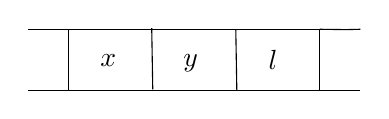
\begin{tikzpicture}[x=0.75pt,y=0.75pt,yscale=-1,xscale=1]
			%Shape: Rectangle [id:dp5885540068356445] 
			\draw   (100,131) -- (221,131) -- (221,160.5) -- (100,160.5) -- cycle ;
			%Straight Lines [id:da9656787853676311] 
			\draw    (140,130.5) -- (140.5,160) ;
			%Straight Lines [id:da799310409405484] 
			\draw    (180.5,131) -- (181,160.5) ;
			%Straight Lines [id:da26873040715798246] 
			\draw    (80.5,131) -- (100,131) ;
			%Straight Lines [id:da10246435939686227] 
			\draw    (80.5,160.5) -- (90.58,160.5) -- (100,160.5) ;
			%Straight Lines [id:da8283986052160006] 
			\draw    (221,160.5) -- (231.08,160.5) -- (240.5,160.5) ;
			%Straight Lines [id:da891243195079455] 
			\draw    (221,131) -- (233.58,131.17) -- (240.5,131) ;
			% Text Node
			\draw (114,141.9) node [anchor=north west][inner sep=0.75pt]    {$x$};
			% Text Node
			\draw (154,141.9) node [anchor=north west][inner sep=0.75pt]    {$y$};
			% Text Node
			\draw (195,139.9) node [anchor=north west][inner sep=0.75pt]    {$l$};
		\end{tikzpicture}
	\end{figure}
	\begin{itemize}
		\item $x$: az adott cella sorának indexe
		\item $y$: az adott cella oszlopának indexe
		\item $l$: 1, ha az $(x,y)$ cella \mintinline{java}|tipTile(Player player)| metódusa igazat adott vissza, különben nulla
	\end{itemize}
	Az üzenet kezelése a játék nézetének (pl. GUI, parancssori kezelőfelület) felelőssége.
	\\[8pt]
	Az \mintinline{java}|getCurrentPlayer()| metódus visszaadja a jelenleg aktív játékost reprezentáló objektum referenciáját \mintinline{java}|getCurrentPlayerIndex()|, pedig ugyanezen játékos \mintinline{java}|players| tömbbeli indexét.
	Az \mintinline{java}|isOver()| metódus igazat ad vissza ha a játék véget ért azaz a játékosok pontszámának összege megegyezik a tábla méretének négyzetével.
	A \mintinline{java}|getWinner()| metódus visszaadja a több pontot elérő \mintinline{java}|players|-beli indexét. Döntetlen esetén (bár ez csak akkor lenne lehetséges ha páros méretű pályák is lennének) 1-et azaz a második játékos indexét adja vissza.
	\subsubsection{GameGUI}
	A \mintinline{java}|GameGUI| osztály felelős a játék kezelőfelületének megvalósításáért. Annak érdekében hogy a játék könnyen újraindítható legyen az osztály konstruktora csak az állandó komponenseket hozza létre. \\[4pt]
	A többi komponens és a játék logikájának elindítása a \mintinline{java}|setupGame(int boardSize)| feladata. A játék végén automatikusan lefut a \mintinline{java}|reset()| metódus, mely alaphelyzetbe állítja a játékot.
	A GUI főbb komponensei:
	\begin{itemize}
		\item új játék menü
		\item tábla (\mintinline{java}|JButton[][] board|)
		\item pontszámlálók (\mintinline{java}|JLabel[] scoreLabels|)
		\item körjelző (\mintinline{java}|JLabel turnLabel|)
	\end{itemize}
	A konstruktorban létrejövő \mintinline{java}|JButton|-ökhöz mind megtalálható \mintinline{java}|ButtonListener| eseménykezelőt. Ezen osztály \mintinline{java}|actionPerformed()| metódusa kommunikál a \mintinline{java}|GameModel| osztállyal, úgy a következő módon:
	\begin{enumerate}
		\item lekéri a jelenlegi játékost
		\item meghívja a cella \mintinline{java}|tipTile(Player player)| metódusát, és feldolgozza az ebből kapott üzenetet:
		\begin{enumerate}
			\item Ha egy cella értéke 4 lett átszínezi a gombot az adott játékos színére, kikapcsolja a gombot és leszedi az eseménykezelőt, frissíti az eredményjelzőt.
			\item Frissíti a gomb szövegét a cella értékére
		\end{enumerate}
		\item lépteti a kört a megfelelő metódussal, frissíti a körjelzőt
		\item ellenőrzi tart-e még a játék az \mintinline{java}|isOver()| metódussal.
	\end{enumerate}
	
	\subsubsection{Game}
	A program fő osztálya, melynek egyetlen feladata egy \mintinline{java}|GameGUI| objektum példányosítása.
	\subsection{UML osztálydiagram}
	\begin{figure}[H]
		\centering
		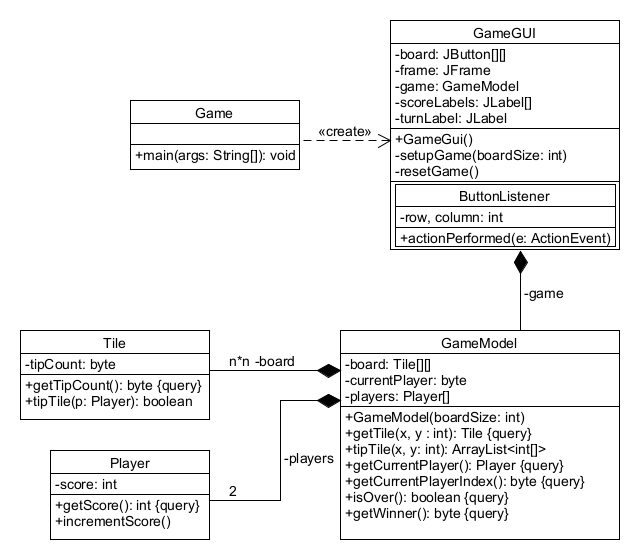
\includegraphics[scale=0.6]{class.png}
	\end{figure}
	\subsection{Implementálás}
	A terv implementálását a \mintinline{java}|Tile| és \mintinline{java}|Player| osztályoktól érdemes kezdeni felfelé haladva.
	\textbf{Java verzió: 17.0.4.1}
	\newpage
	\section{Tesztelés}
	\subsection{Fehérdobozos tesztesetek}
	\begin{tabularx}{\textwidth}{|Y|Y|Y|}
		\hline
		Leírás & Tevékenység & Elvárt eredmény \\
		\hline
		Cella pöccintés cella értéke nem négy lesz & tile.tipTile() & Hamis \\
		\hline
		Cella pöccintés cella értéke négy lesz & tile.tipTile() & Igaz \\
		\hline
		Cella pöccintés cella értéke már volt négy & tile.tipTile() & Hamis \\
		\hline
		Cella értéke nem lehet több mint négy& tile.tipTile() & tile.getTipCount()==4 \\
		\hline
		Illegális tábla méret & GameModel() & IllegalArgumentException \\
		\hline
	\end{tabularx}
	\\[4pt]
	Fehérdobozos tesztesetekhez JUnit 4.13-as tesztkörnyezet: \textbf{GameTest.java}
	\subsection{Feketedobozos tesztesetek}
	\begin{tabularx}{\textwidth}{|Y|Y|}
		\hline
		Tevékenység & Elvárt eredmény \\
		\hline
		Program elindítása & Létrejön ablak a táblaméret választó menüvel \\
		\hline
		Új játék létrehozása a menüből & Létrejönnek a GUI komponensek, elindul a játék \\
		\hline
		Kattintás cellára & A cella és környező cellák értéke megváltozik, a játékos köre véget ér \\
		\hline
		Egy cella értéke 4 lesz & Az átpöccintő játékos pontszámának növelése, gomb kikapcsolása és átszínezése \\
		\hline
		Új játék létrehozása, úgy hogy, folyamatban van játék & Új GUI komponensek jönnek létre, új játék indul \\
		\hline
		Játék véget ér & Párbeszédablak jelenik meg, ami kiírja a nyertest \\
		\hline
		Párbeszédablak bezárása & Új játék indul \\
		\hline
	\end{tabularx}
\end{document}